\documentclass{article}
\usepackage[T1]{fontenc}
\usepackage[a4paper, margin=1in]{geometry}
\usepackage[utf8]{inputenc}
\usepackage{amsmath, amssymb, graphicx, hyperref}
\graphicspath{{../figures/}}
\usepackage{bookmark}
\usepackage[framed,numbered]{matlab-prettifier}
\usepackage{xcolor}
\usepackage{listings}

\geometry{a4paper, margin=1in}

% MATLAB code style
\lstset{
  style      = Matlab-editor,
  basicstyle = \mlttfamily,
  breaklines = true
}

\title{\textbf{Practical - 5}}
\author{}
\date{October 17, 2026}

\pagenumbering{gobble}

\begin{document}
\maketitle

\noindent
\textbf{\large{Aim:}} To plot the solution family of a higher-order differential equation.

\vspace{1em}
\noindent
\textbf{\large{MATLAB Code:}}

\begin{lstlisting}
clc; clear  all; close all;

syms y(x)

eqn = diff(y,4) == 0;
ySol = dsolve(eqn);

disp('General solution:')
disp(ySol)

hold on
fplot(subs(ySol, {'C1', 'C2', 'C3', 'C4'},{0, 1, 0, 0}), [-3 3], 'LineWidth',1.5)
fplot(subs(ySol, {'C1', 'C2', 'C3', 'C4'},{1, 1, 0, 0}), [-3 3], 'LineWidth',1.5)
fplot(subs(ySol, {'C1', 'C2', 'C3', 'C4'},{0, 0, 1, 0}), [-3 3], 'LineWidth',1.5)
fplot(subs(ySol, {'C1', 'C2', 'C3', 'C4'},{1, 0, 0, 1}), [-3 3], 'LineWidth',1.5)

grid on
xlabel('x')
ylabel('y(x)')
title('Family of Solutions of d^4y/dx^4 = 0')
legend('y = x', 'y = 1 + x', ...
'y = x^2', 'y = 1 + x^3', ...
'Location','best')
hold off

\end{lstlisting}

\vspace{1em}
\noindent
\textbf{\large{Output:}}

\begin{flushleft}
    \tiny{General Solution:}
\end{flushleft}

\begin{flushleft}
    $\frac{C_1 \,x^3 }{6}+\frac{C_2 \,x^2 }{2}+C_3 \,x+C_4$
\end{flushleft}

\newpage
\begin{figure}[htbp]
    \centering
    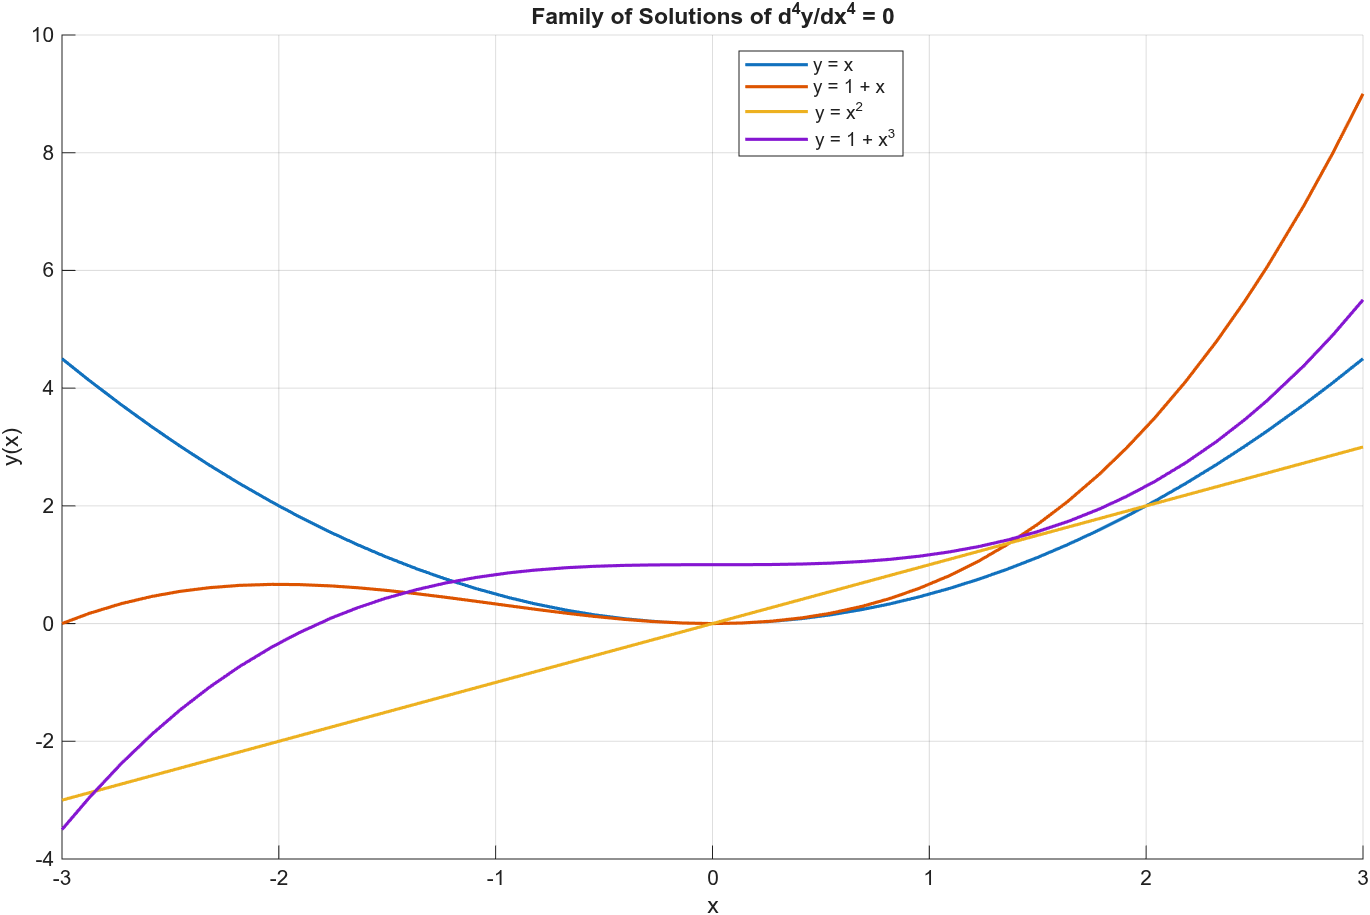
\includegraphics[width=0.7\textwidth]{Figure5.png}
\end{figure}

\end{document}
